\todo[inline]{Onde colocar detalhes da minha implementação?}
Este capítulo apresentará o método proposto por este trabalho para o desenvolvimento de um simulador de prótese ativa baseada em sensores e aprendizado de máquina.

\section{Visão geral do método}\label{sec:metodo_protese}

Este trabalho apresenta um simulador de prótese robótica para membros inferiores ou, mais especificamente, para as articulações do pé, visando prover suporte para a construção de modelos de próteses, aproveitando-se para simular as partes mecânicas articuladas e a inclusão de cenários de diferentes tipos de superfícies.

O simulador foi projetado para funcionar como uma prótese transtibial, ou seja, para pernas que contenham a articulação do joelho intacta, atuando sobre a rigidez de suas articulações para adaptá-la a diferentes situações. Isto é possível pois a simulação conta ainda com a utilização de um classificador de movimentos capaz de prever as ações necessárias nas partes mecânicas através da coleta de dados de sensores em um dispositivo vestível na forma de joelheira.

Este dispositivo está equipado com sensores flexíveis \cite{flex:datasheet} nas articulações dos joelhos além de giroscópios e acelerômetros \cite{invensense:imu_mpu}, que serão usados para capturar as ações do usuário. A \autoref{fig:big_picture_prosthesis} ilustra a visão geral do sistema, incluindo o posicionamento dos sensores para o simulador juntamente com uma possível prótese implementada com atuadores reais (\autoref{fig:big_picture_prosthesis}) e a simulação gerada a partir dos dados coletados dos sensores, com a movimentação do pé a partir da classificação destes dados (\autoref{fig:simulation_prototype}).

% \begin{figure}[h]
% 	\caption{\label{fig:big_picture}Visão geral do protótipo}
% 	\begin{center}
% 	    \fbox{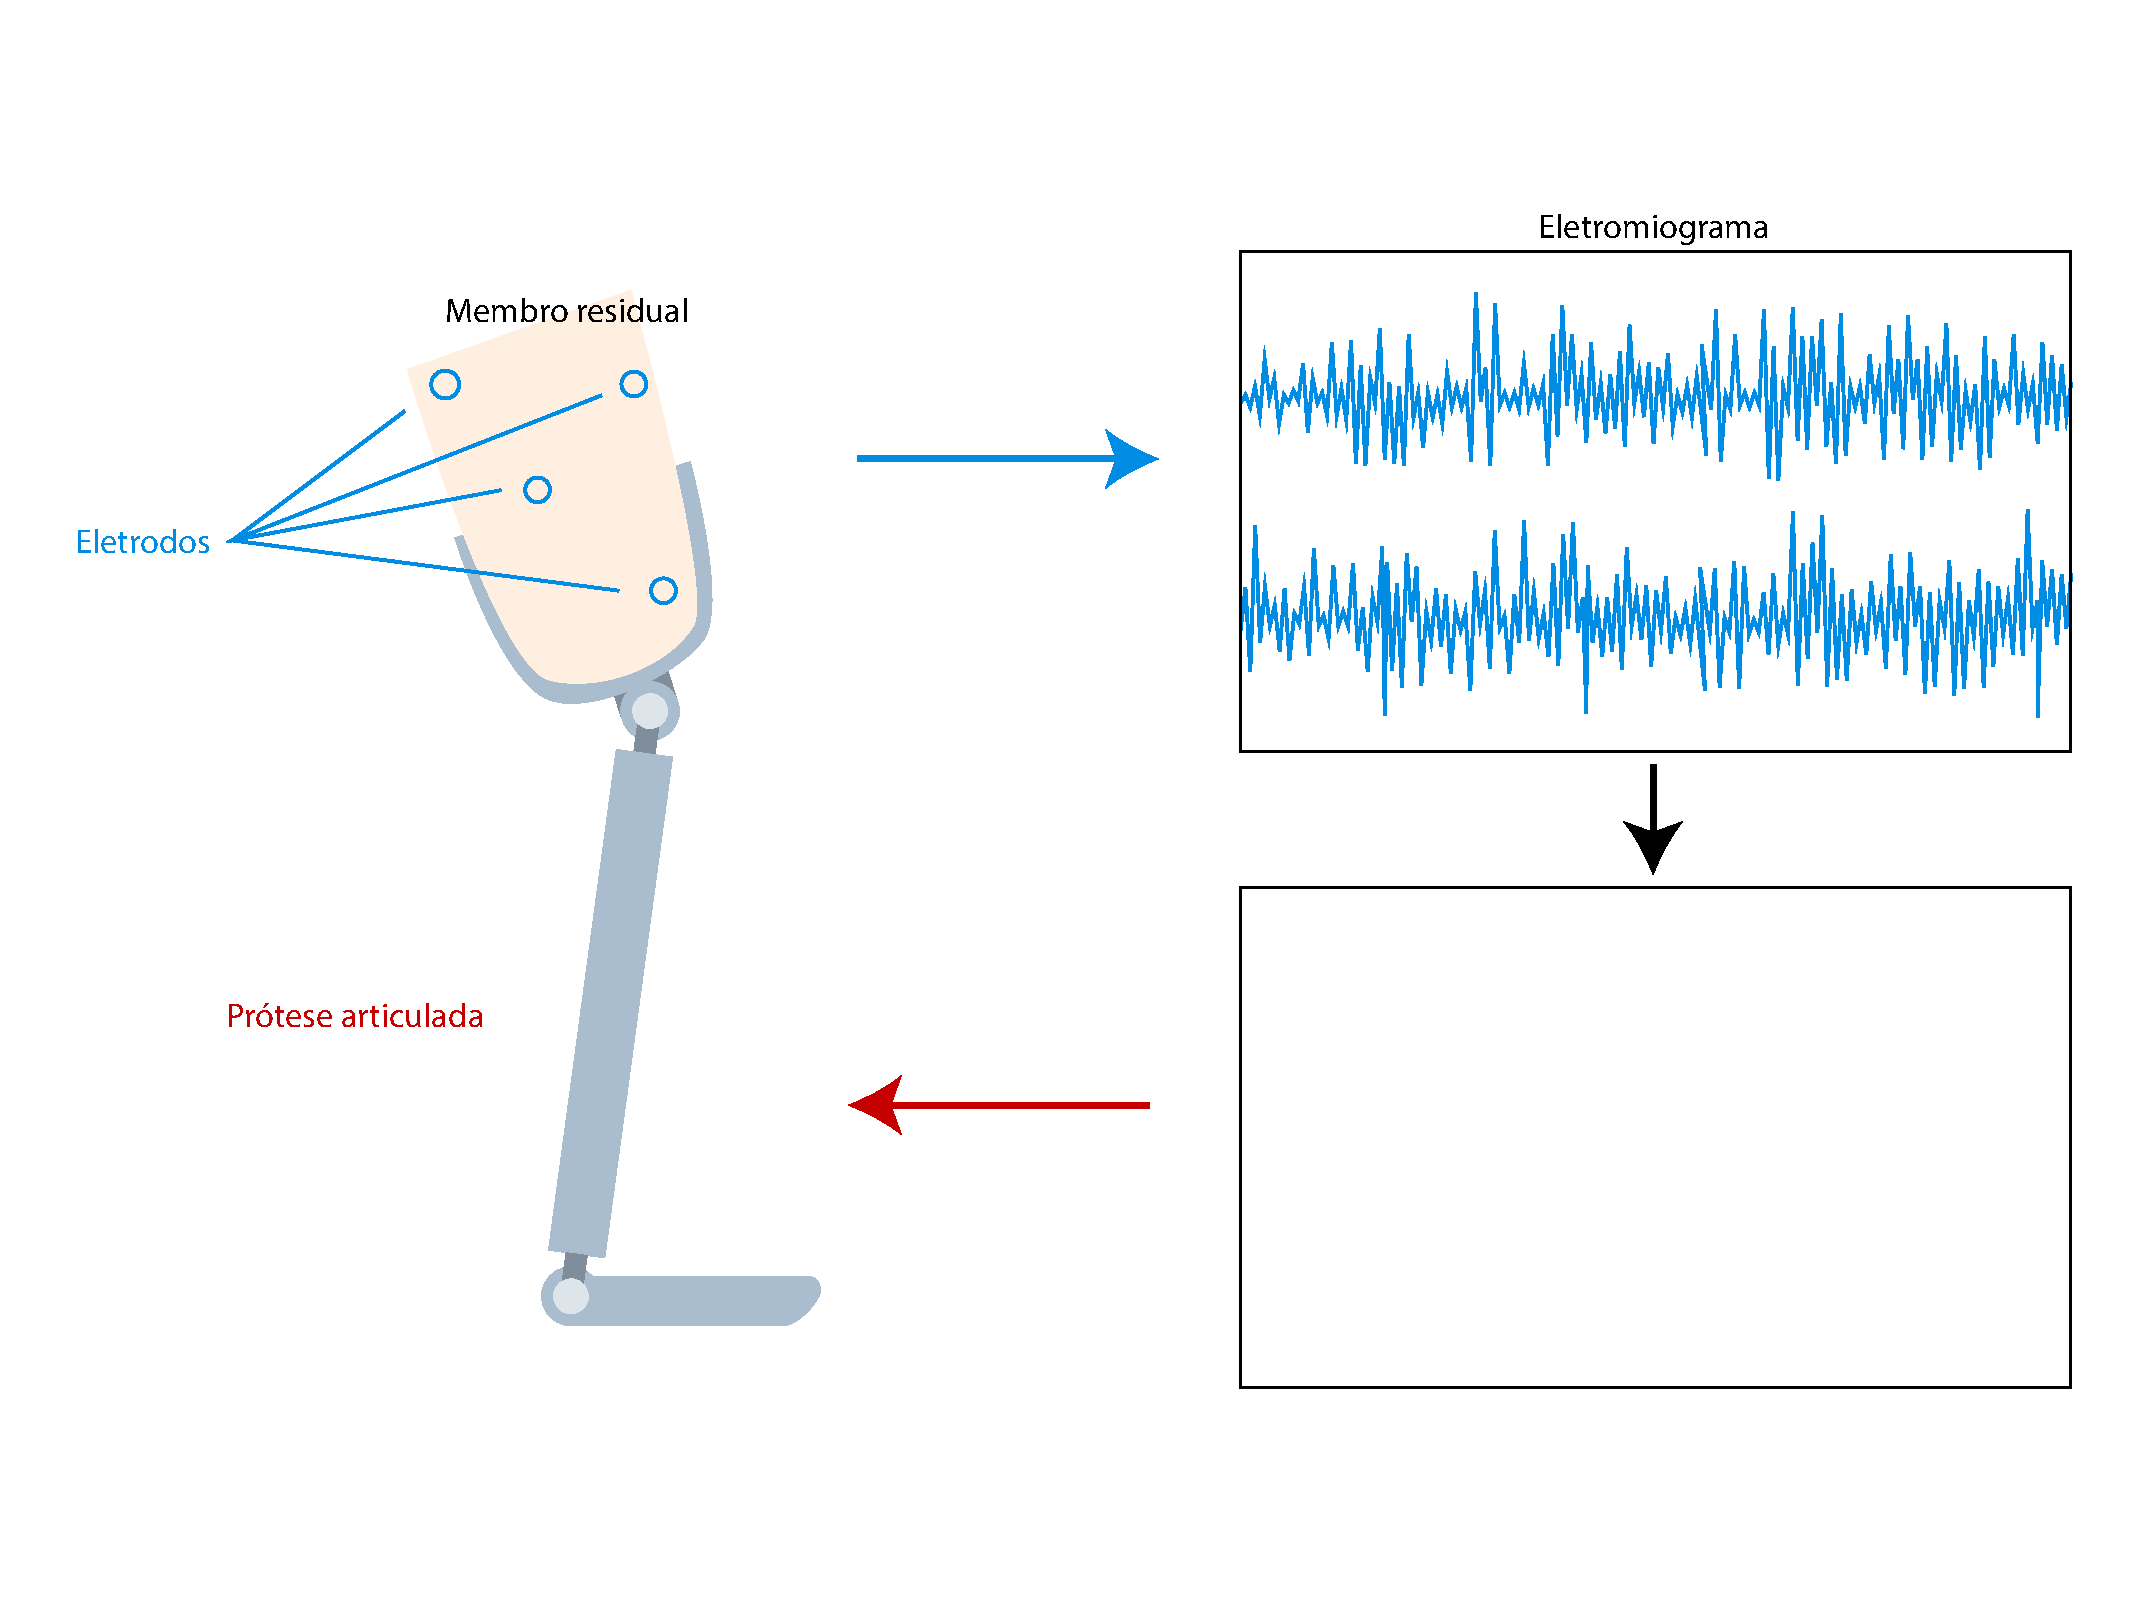
\includegraphics[width=0.6\textwidth]{resources/big_picture}}
% 	\end{center}
% 	\legend{Fonte: Elaborada pelo autor}
% \end{figure}

\begin{figure}[ht]
    \centering
    \caption{Visão geral do sistema}
    \label{fig:big_picture}
    \subfloat[Proposta de implementação de prótese\label{fig:big_picture_prosthesis}]
        {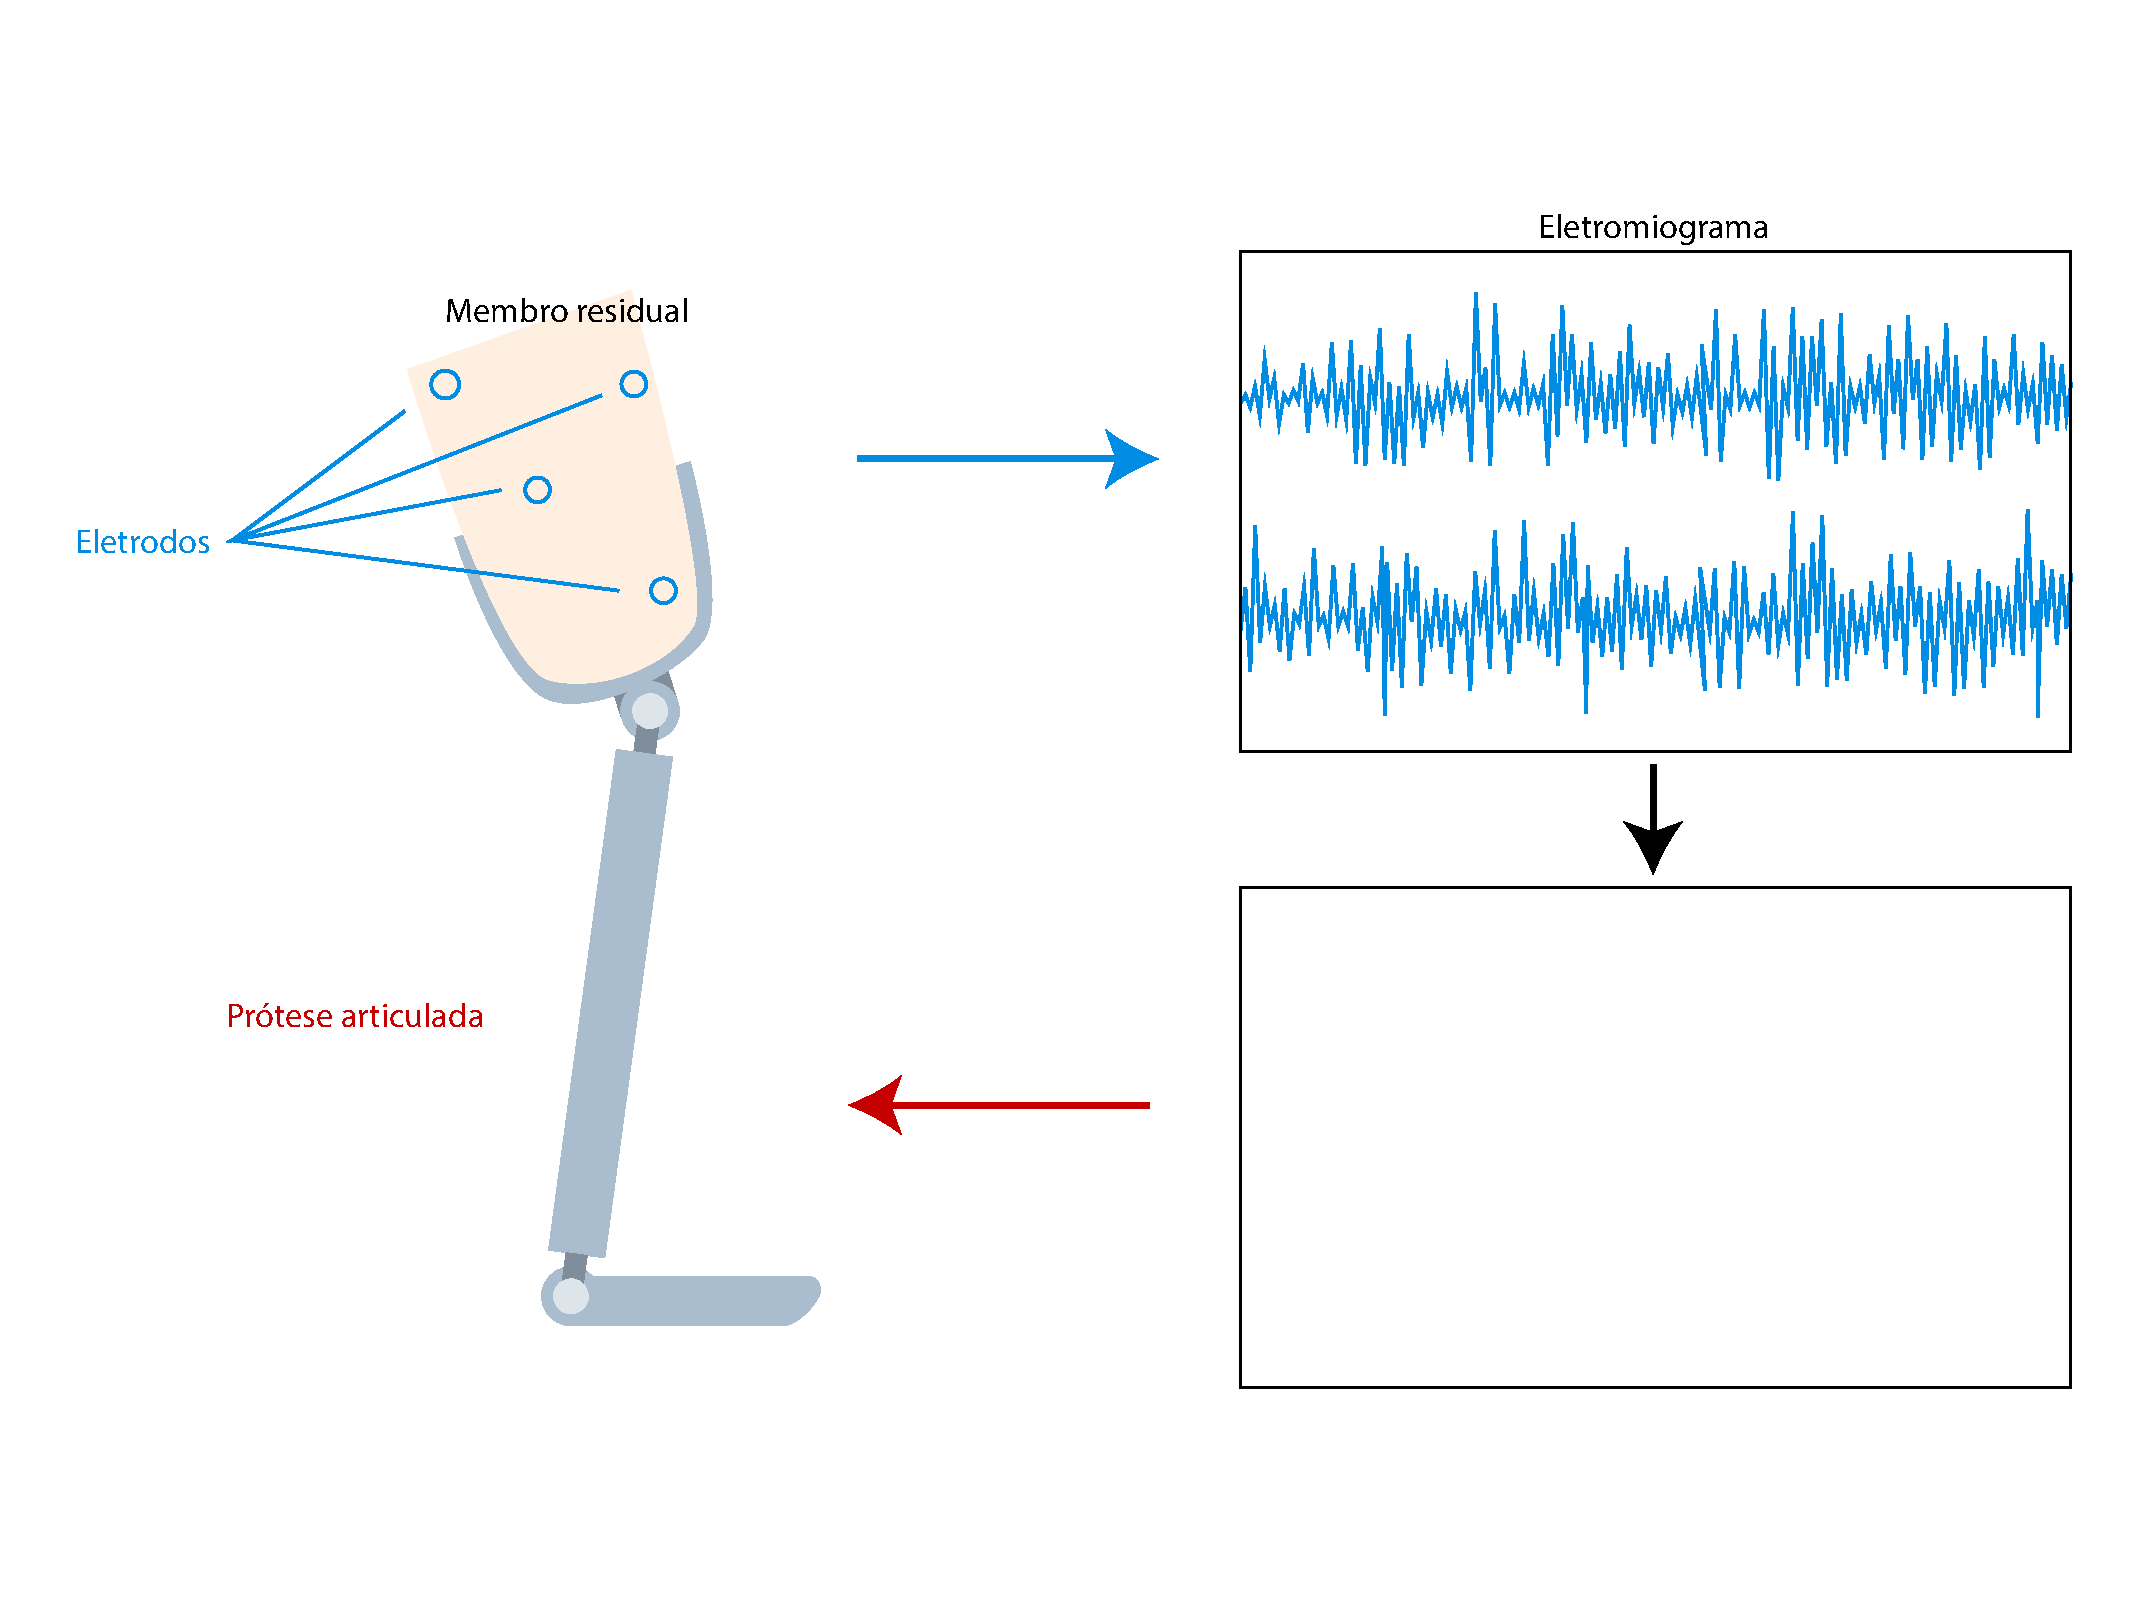
\includegraphics[height=5cm]{resources/big_picture}}
    \hspace{1cm}
    \subfloat[Simulação virtual do protótipo\label{fig:simulation_prototype}]
        {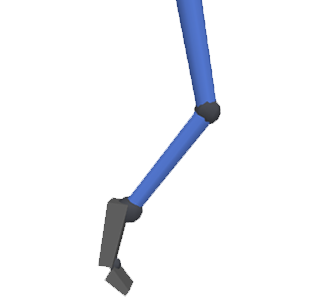
\includegraphics[height=5cm]{resources/method_simulacao}}
    \legend{Fonte: Elaboradas pelo autor}
\end{figure}

No dispositivo vestível, os sensores são posicionados nos joelhos do usuário, e os dados capturados são transmitidos por uma placa de processamento para o simulador em um computador. 
% posicionada na estrutura da própria prótese, que 
O simulador então utiliza os dados enviados para mostrar o modelo virtual, e os classifica para determinar a ação dos atuadores, conforme fluxograma ilustrado na \autoref{fig:flowchart}, em um modelo virtual da prótese em tempo real.
% O fluxo  como pode ser visto no fluxograma ilustrado na \autoref{fig:flowchart}.

\begin{figure}[ht]
	\caption{\label{fig:flowchart}Fluxograma da coleta de dados para o simulador}
	\begin{center}
	    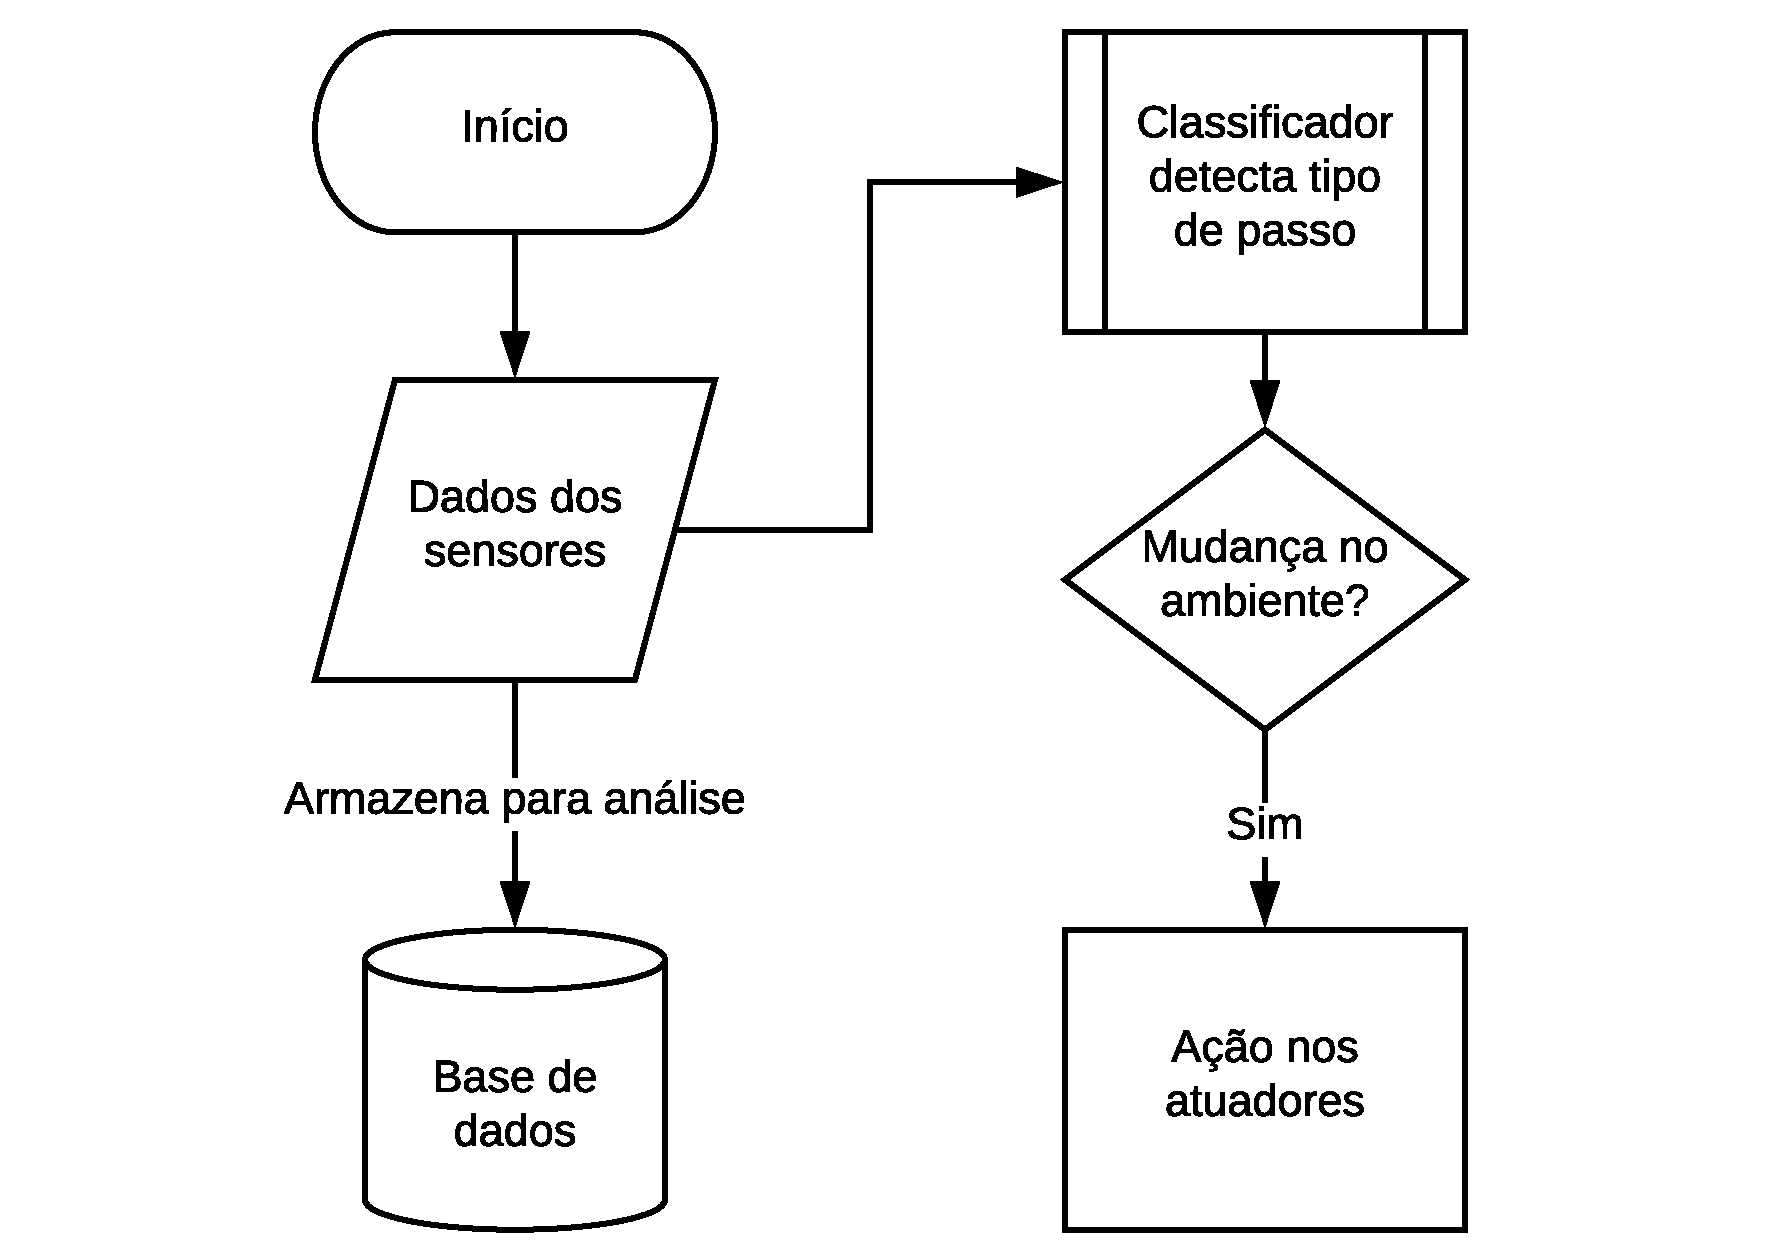
\includegraphics[width=0.8\textwidth]{resources/flowchart}
	\end{center}
	\legend{Fonte: Elaborada pelo autor}
\end{figure}


\section{Prototipação da prótese no simulador}\label{sec:metodo_prototipacao}

O diagrama de sequência da \autoref{fig:sequence_diagram} representa os componentes do sistema proposto por este trabalho, bem como a interação entre eles. Nela, pode-se observar a presença dos objetos caracterizados como \textbf{Sensores} com fio e sem fio e \textbf{Central de \textit{hardware}}, que compõem o dispositivo vestível, e \textbf{Simulação} que representa a visualização do modelo da perna e da prótese no computador.
% O wearable também pode ser utilizado são os localizados no membro intacto do usuário, que devem se transmitir os dados à central de processamento na prótese.

\begin{figure}[ht]
	\caption{\label{fig:sequence_diagram}Diagrama de sequência que descreve a interação entre os componentes do sistema}
	\begin{center}
	    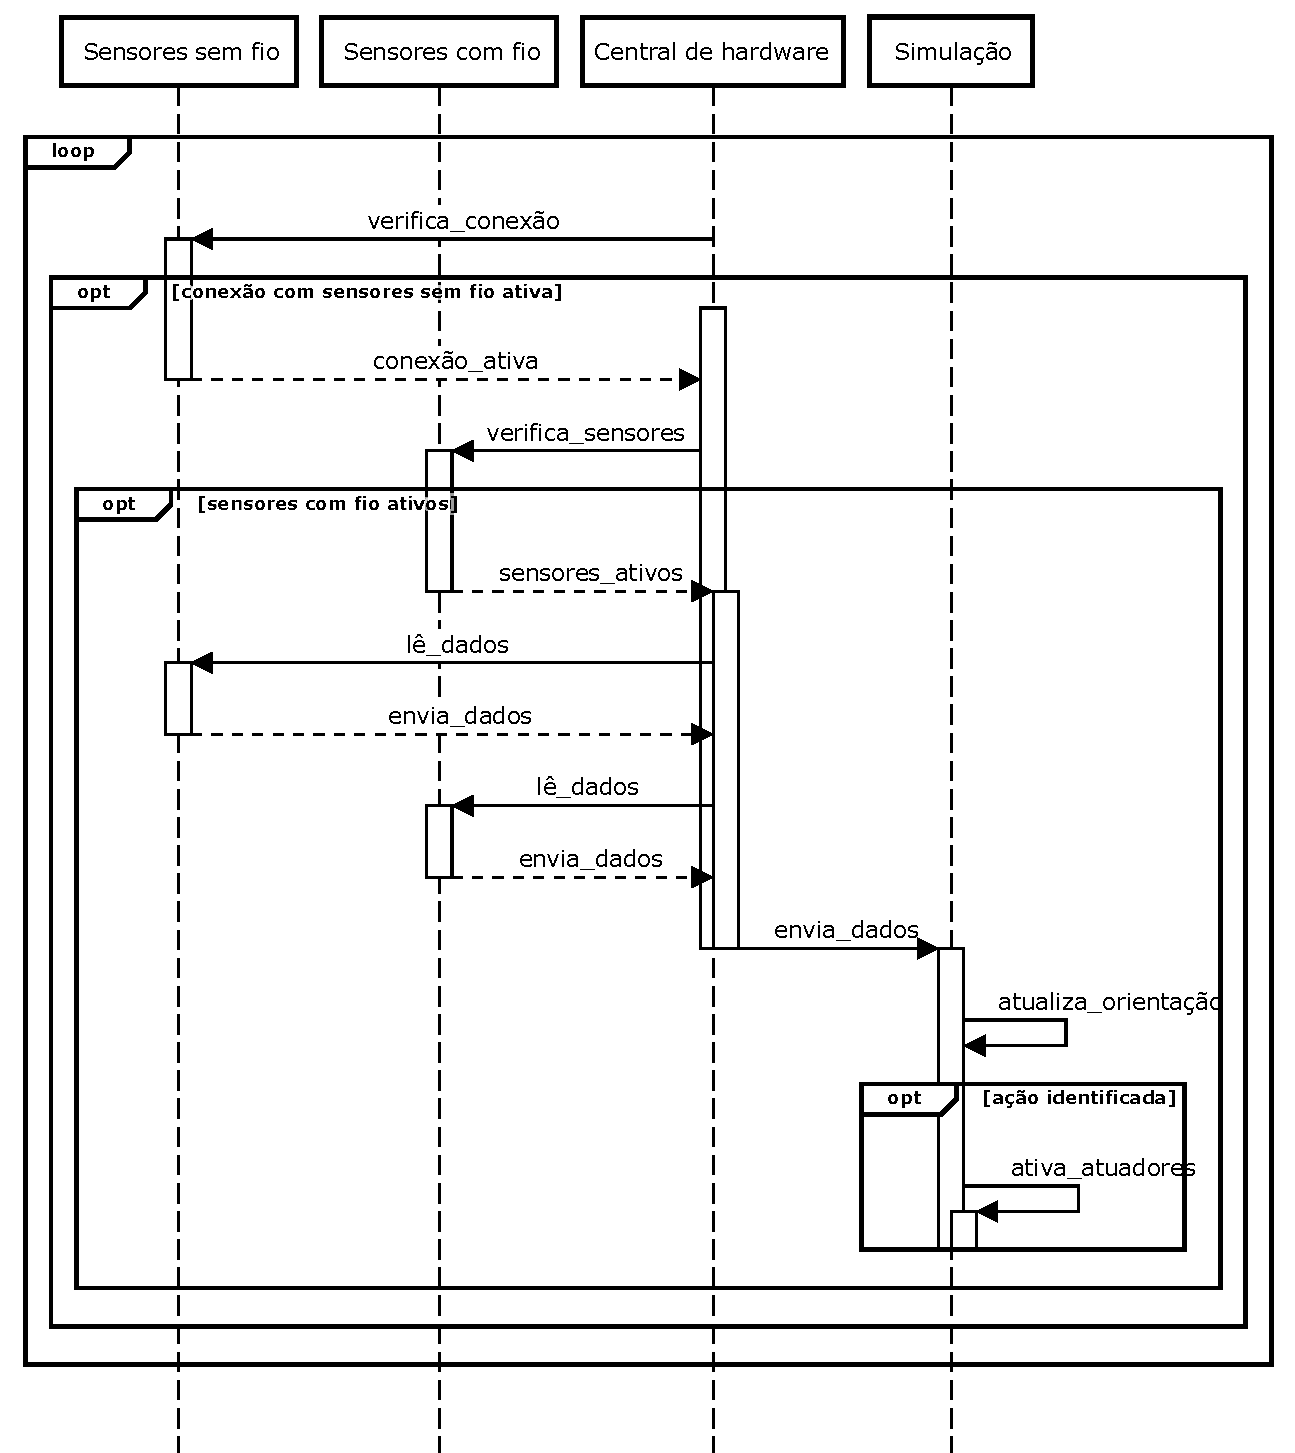
\includegraphics[width=\textwidth]{resources/sequence_diagram}
	\end{center}
	\legend{Fonte: Elaborada pelo autor}
\end{figure}

A central localizada na perna da prótese recebe os dados de todos os sensores de forma constante e dados são então repassados à simulação, que os utiliza para orientar a posição da perna virtual de acordo com os dados dos giroscópios e acelerômetros e para classificar os movimentos, o que a permite que realize ações sobre as articulações da prótese virtual de acordo com o movimento detectado como, por exemplo, caso tenha sido iniciado um passo.

% \subsection{Arquitetura do \textit{software}}\label{sec:metodo_prot_software}
% O \textit{software} relativo à~\autoref{fig:sequence_diagram} será modelado através de uma rede de Petri. Desta forma, será possível validar o sistema para garantir confiabilidade. Esta validação será feita conforme as propriedades descritas na Seção~\ref{sec:petrinet}, como segurança e vivacidade, além de possivelmente outras propriedades adicionais. 
% % 
% Vale ressaltar que a transformação do diagrama de sequência para rede de petri de forma automatizada é possível utilizando ferramentas como o FOREVER~\cite{cunha:2011forever}.\todo{Manter isso sobre rede de Petri?}
% 
% A classificação será realizada com a utilização de uma ferramenta como as descritas na Seção~\ref{sec:ml_tools}. Além disso, será necessário fazer o treinamento do algoritmo de classificação, para que se tenha um protótipo funcional. Inicialmente, o \textit{software} para treinamento será produzido separadamente ao sistema de classificação principal, de modo a se criar um conjunto de dados a ser usado pela classificação na prótese.

\subsection{Arquitetura de \textit{hardware} proposta}\label{sec:metodo_prot_hardware}
A prótese virtual é apresentada em um modelo virtual 3D que simula a ação dos atuadores ao prever os movimentos e conta com duas articulações ativas no pé, como visto na~\autoref{fig:simulation_prototype}. O intuito deste modelo é proporcionar o futuro uso de uma impressora 3D para construção de uma prótese física. O uso de impressão 3D tem o intuito de manter o baixo custo do produto.

A~\autoref{fig:hardware_scheme} mostra o funcionamento dos atuadores de um modelo proposto de prótese que se beneficiaria deste sistema, com atuadores que deverão ser acionados de acordo com a classificação dos dados dos sensores. No ponto \textbf{A}, o motor do tornozelo da prótese regula a rigidez da articulação, como forma de manter estabilidade nos passos. Os pontos \textbf{B} e \textbf{C} referem-se a motores de passo que, juntos a hastes, se prendem no calcanhar da prótese, para mover o pé e exercer força na pisada.

\begin{figure}[ht]
	\caption{\label{fig:hardware_scheme}Esquema representando o funcionamento dos atuadores}
	\begin{center}
	   \fbox{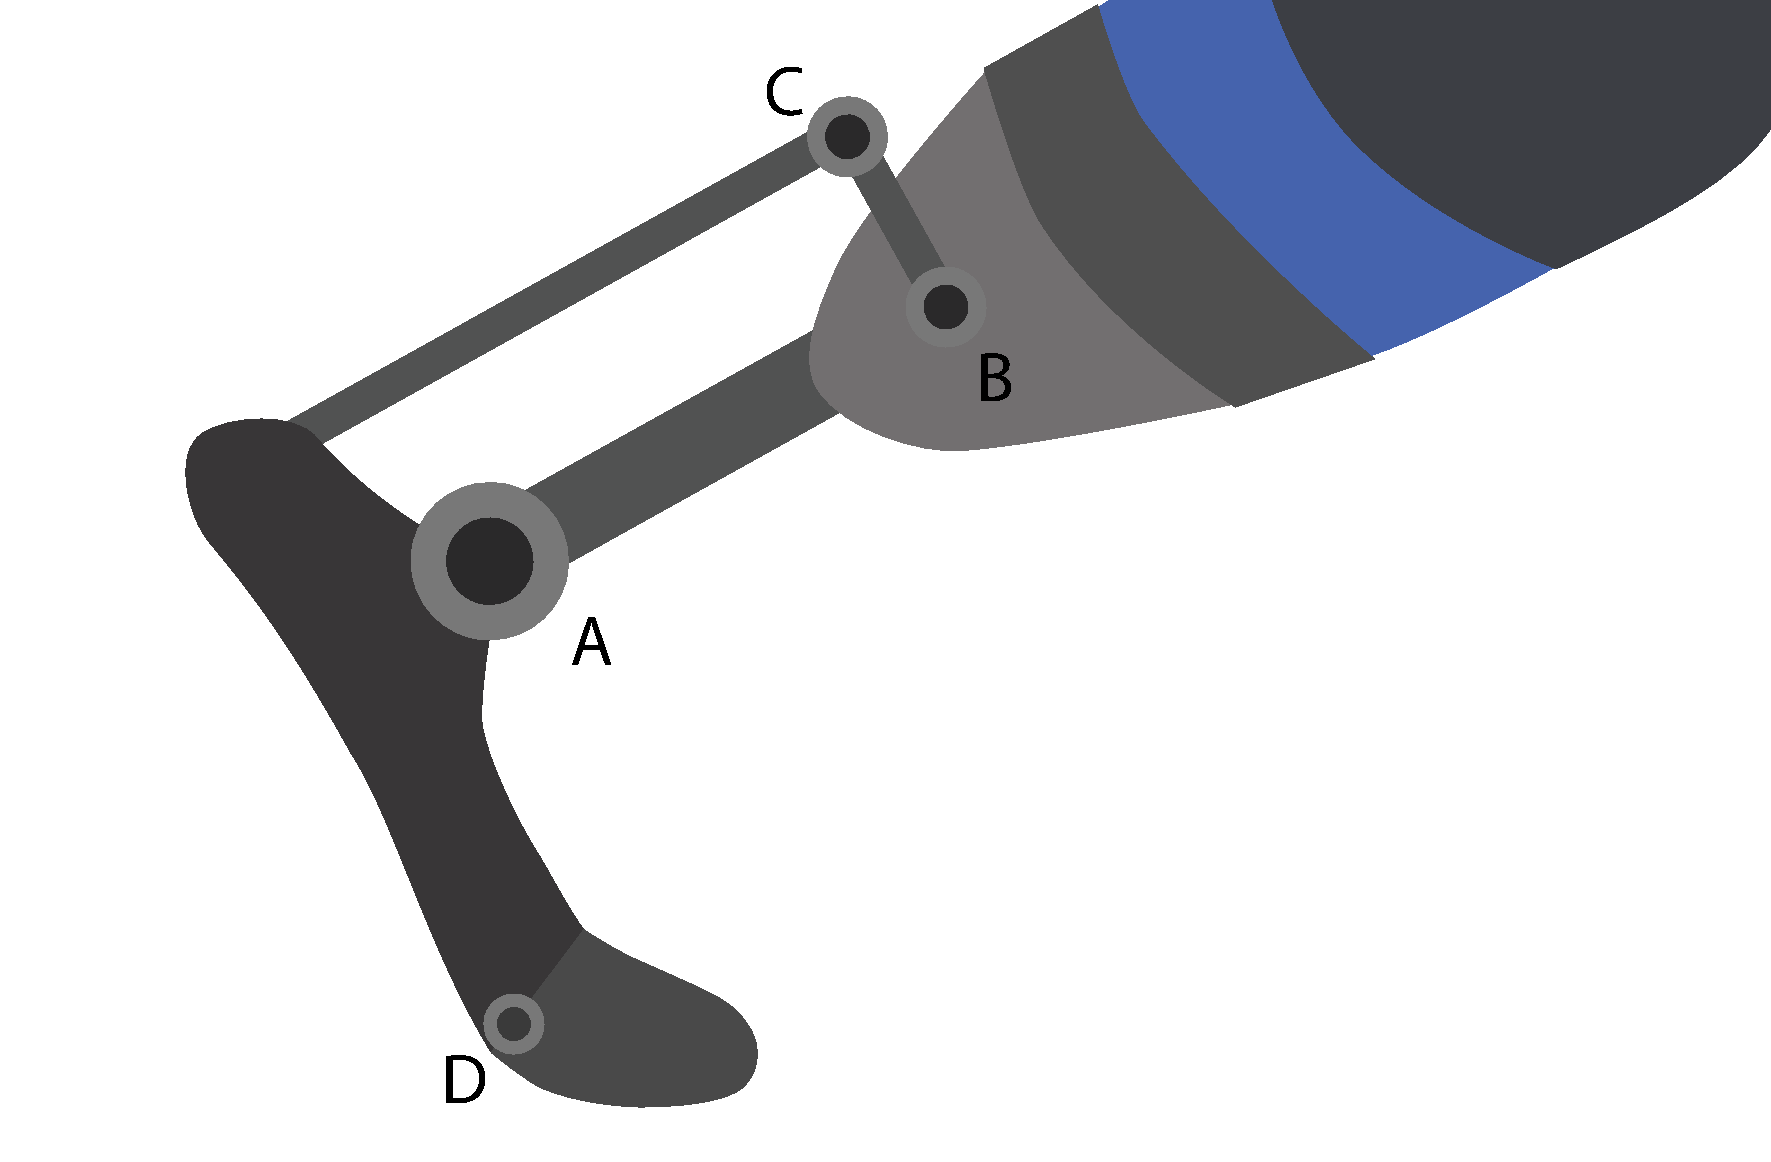
\includegraphics[width=0.5\textwidth]{resources/hardware_scheme}}	   %\missingfigure[figwidth=12cm,figheight=8cm]{Desenho de detalhe da prótese, com articulações, motores, etc.}
	\end{center}
	\legend{Fonte: Elaborada pelo autor}
\end{figure}

Por fim, o ponto \textbf{D} da \autoref{fig:hardware_scheme} é uma articulação motorizada que manipula a parte dianteira do pé, a fim de controlar a curvatura, simulando a flexibilidade de um pé humano. Alguns exemplos de configurações possíveis dos motores e articulações de acordo com diferentes cenários serão mostrados posteriormente na \autoref{fig:hardware_poses}. Deve-se salientar que este é um modelo de prótese proposto neste trabalho, contudo o simulador pode ser adaptado também a outros modelos.


% \section{Coleta de dados}\label{sec:metodo_coleta}
% 
% \todo[inline]{Somente um sensor}
% Para que o sistema possa analisar e classificar os movimentos conforme a prótese é acioanda normalmente, serão utilizados sensores nas duas pernas. Em cada joelho será posicionado um conjunto de um sensor flexível, um giroscópio e um acelerômetro, que serão utilizados em conjunto.
% 
% %\todo{Adicionar um exemplo de dados gerados pelos sensores}
% Os valores capturados pelos sensores do membro intacto serão transmitidos sem fios para a central de classificação dos sinais, que se conecta aos atuadores. Os sensores posicionados no membro residual se comunicarão diretamente através de fios com a central, pois estão posicionados fisicamente próximos. Os dados também serão armazenados para a análise descrita na Seção~\ref{sec:metodo_diagnostico}.

\section{Previsão de movimentos no simulador}\label{sec:metodo_previsao}

% \todo[inline]{Mudar a previsão de movimentos, já que não usa a perna intacta?}
Os dados coletados são analisados por um algoritmo de aprendizado de máquina para que se classifique e se preveja as ações do usuário. Essas ações são classificadas de acordo com o passo a ser dado, podendo ser caminhada plana, subida ou descida de degrau. Enquanto o usuário realiza um passo, o sistema deverá identificar em que ambiente este passo será dado. Isto poderá ser feito a partir do passo anterior, e a partir do movimento atual extraído do dispositivo vestível posicionado no membro residual que se está analisando.

Considerando que haverá um conjunto predeterminado de cenários possíveis -- caminhada plana, subida e descida de escada -- a técnica de aprendizado de máquina supervisionado para classificação utilizada no simulador é a XX\todo{Confirmar o nome da técnica}, conforme analisado em testes preliminares feitos e apresentados na \autoref{sec:result_execucao}. Quando o tipo de passo a ser realizado é identificado pelo sistema, acionam-se os atuadores, que terão sua ação determinada de acordo com o cenário identificado. Na~\autoref{fig:hardware_poses} pode-se observar a forma em que a prótese deve se posicionar de acordo com cada tipo de ação. As ações diferem para o início e o fim de cada passo em diferentes cenários.

As três ações representadas na \autoref{fig:hardware_poses} referem-se a (a) pisada plana, (b) fim de um passo em piso plano, e (c) descida de escada. No primeiro caso, os motores só mantêm estabilidade para garantir equilíbrio; no segundo caso, é necessária maleabilidade na dianteira do pé, para que seja possível impulsionar o passo do usuário. No terceiro caso, antes que o usuário desça o próximo degrau, a prótese deve inclinar-se e contrair a dianteira do pé para evitar tropeços e auxiliar na descida.

\begin{figure}[h]
	\caption{\label{fig:hardware_poses}Algumas posições da prótese de acordo com cenários distintos}
	\begin{center}
	   \fbox{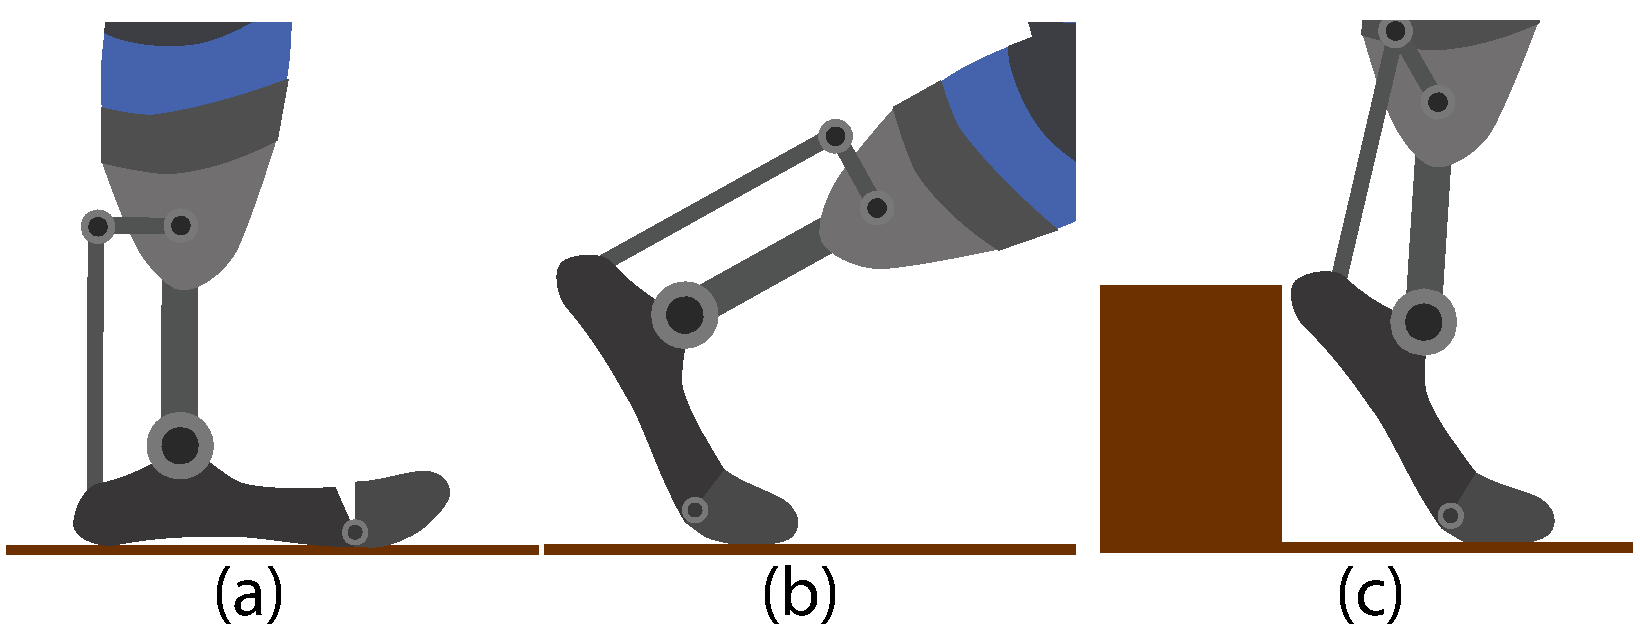
\includegraphics[width=\textwidth]{resources/hardware_poses}}
	   %\missingfigure[figwidth=12cm,figheight=5cm]{Poses da prótese em diferentes situações: início de caminhada, fim de caminhada, descida de escada.}
	\end{center}
	\legend{Fonte: Elaborada pelo autor}
\end{figure}


\section{Diagnóstico do uso da prótese e recomendações de melhorias no caminhar}\label{sec:metodo_diagnostico}

Os dados dos sensores também poderão ser armazenados para geração de estatísticas que podem ser usadas para diagnóstico relacionado à saúde da caminhada do futuro usuário da prótese~\cite{SabatiniMSC05}.
% O sistema fará um relatório do uso, indicando se é exercida mais força em uma das pernas do que na outra, por exemplo, além de outros dados.
A partir das informações geradas, poderão ser feitas recomendações de melhorias ao indivíduo, via consulta a um especialista, para que se melhore a postura, a caminhada, ou que se utilize algum tipo de equipamento adicional. 
% Além disso, ainda será possível analisar as estatísticas de uso da prótese para avaliar seu impacto na vida do usuário, caso esteja alterando seus hábitos de alguma forma.

Como trabalho futuro, pretende-se adicionar ao simulador um analisador de eficácia da prótese em relação aos sensores utilizados na joelheira para simulação da prótese, visto que tais sensores poderão ser utilizados na prototipação de uma prótese física. Para que este diagnóstico seja possível, será analisada a hipótese do uso de sensores adicionais aos definidos pelo protótipo atual, caso estes não sejam suficientes para gerar os dados necessários de análise de saúde da caminhada.